\documentclass[a4paper,12pt]{article}
\usepackage{xcolor}
\usepackage{amsmath,amsfonts,amssymb}
\usepackage{geometry}
\usepackage{fancyhdr}
\usepackage{graphicx}
\usepackage{titlesec}
\usepackage{tikz}
\usepackage{booktabs}
\usepackage{array}
\usetikzlibrary{shadows}
\usepackage{tcolorbox}
\usepackage{float}
\usepackage{lipsum}
\usepackage{mdframed}
\usepackage{pagecolor}
\usepackage{mathpazo}   % Palatino font (serif)
\usepackage{microtype}  % Better typography

% Page background color
\pagecolor{gray!10!white}

% Geometry settings
\geometry{margin=0.5in}
\pagestyle{fancy}
\fancyhf{}

% Fancy header and footer
\fancyhead[C]{\textbf{\color{blue!80}CS754 Assignment-1}}
% \fancyhead[R]{\color{blue!80}Saksham Rathi}
\fancyfoot[C]{\thepage}

% Custom Section Color and Format with Sans-serif font
\titleformat{\section}
{\sffamily\color{purple!90!black}\normalfont\Large\bfseries}
{\thesection}{1em}{}

% Custom subsection format
\titleformat{\subsection}
{\sffamily\color{cyan!80!black}\normalfont\large\bfseries}
{\thesubsection}{1em}{}

% Stylish Title with TikZ (Enhanced with gradient)
\newcommand{\cooltitle}[1]{%
  \begin{tikzpicture}
    \node[fill=blue!20,rounded corners=10pt,inner sep=12pt, drop shadow, top color=blue!50, bottom color=blue!30] (box)
    {\Huge \bfseries \color{black} #1};
  \end{tikzpicture}
}
\usepackage{float} % Add this package

\newenvironment{solution}[2][]{%
    \begin{mdframed}[linecolor=blue!70!black, linewidth=2pt, roundcorner=10pt, backgroundcolor=yellow!10!white, skipabove=12pt, skipbelow=12pt]%
        \textbf{\large #2}
        \par\noindent\rule{\textwidth}{0.4pt}
}{
    \end{mdframed}
}

% Document title
\title{\cooltitle{CS754 Assignment-3}}
\author{{\bf Saksham Rathi, Ekansh Ravi Shankar, Kshitij Vaidya}}
\date{}

\begin{document}
\maketitle
\textbf{Declaration:} The work submitted is our own, and
we have adhered to the principles of academic honesty while completing and submitting this work. We have not referred to any unauthorized sources, and we have not used generative AI tools for the work submitted here.

\section*{Question 2}

\begin{solution}{Solution}

\section{Methodology}

\subsection{Problem Formulation}
The coded snapshot $E_u$ is obtained as:
\[
E_u = \sum_{t=1}^{T} C_t \odot F_t + \eta
\]
where:
\begin{enumerate}
    \item $C_t$ is a binary code modulating frame $F_t$,
    \item $\eta$ is additive Gaussian noise with $\sigma = 2$.
\end{enumerate}

\textbf{Objective:} Given $E_u$ and $\{C_t\}_{t=1}^T$, recover $\{F_t\}_{t=1}^T$.

\subsection{Linear System Representation}
The problem is reformulated as $\mathbf{Ax} = \mathbf{b}$, where:
\begin{enumerate}
    \item $\mathbf{x}$: Vectorized form of all frames $\{F_t\}$,
    \item $\mathbf{b}$: Vectorized coded snapshot $E_u$,
    \item $\mathbf{A}$: Block-row matrix where each block is $\text{diag}(\text{vec}(C_t))$.
    \begin{align}
        A = [diag(C_1) \hspace{5pt} diag(C_2) \cdots diag(C_T)]
    \end{align}
\end{enumerate}

\noindent For \textbf{patch-wise processing} (8$\times$8 patches):
\begin{enumerate}
    \item $\mathbf{x}$: Sparse coefficients of patches in 2D-DCT basis,
    \item $\mathbf{A}$: Constructed as:
    \[
    \mathbf{A} = \begin{bmatrix}
    \text{diag}(\text{vec}(C_1)) \mathbf{\Psi} & \cdots & \text{diag}(\text{vec}(C_T)) \mathbf{\Psi}
    \end{bmatrix}
    \]
    where $\mathbf{\Psi}$ is the 2D-DCT basis.
    \item $\mathbf{b}$: Vectorised patch vector
\end{enumerate}

\subsection{Reconstruction via OMP}
\begin{enumerate}
    \item \textbf{Patch Extraction:}
    \begin{enumerate}
        \item Divide $E_u$ into overlapping 8$\times$8 patches.
        \item For each patch, solve:
        \[
        \mathbf{A}_{\text{patch}} \mathbf{x}_{\text{patch}} = \mathbf{b}_{\text{patch}}
        \]
        using OMP (sparsity constraint: $k = 10$).
    \end{enumerate}
    
    \item \textbf{Sparse Recovery:}
    \begin{enumerate}
        \item OMP iteratively selects the most correlated basis vectors and solves a least-squares problem.
    \end{enumerate}
    
    \item \textbf{Frame Reconstruction:}
    \begin{enumerate}
        \item Reconstruct each patch via $\mathbf{\Psi x}$.
        \item Average overlapping regions to suppress artifacts.
    \end{enumerate}
\end{enumerate}

\subsection{Results}

\noindent To quantify the quality of the reconstruction we computed the RRMSE (Normalised Root Mean Squared Error). A trend that was observed was that the the RRMSE for frames increases on increasing the values of T. This can be explained by the fact that the total information available to us in the long exposure frame remains that same but we are inferring more number of frames from that leading to an increase in the error and decrease in reconstruction quality. 

\end{solution}

\begin{table}[htbp]
  \centering
  \label{tab:rmse}
  \begin{tabular}{|l|c|}
    \hline
    \textbf{Image Identification} & \textbf{RMSE} \\
    \hline
    Cars T = 3 & 0.7915 \\
    Cars T = 5 & 0.8056 \\
    Cars T = 7 & 0.8107 \\
    Flame T = 5 & 1.1015 \\
    \hline
  \end{tabular}
  \caption{Mean RMSE Values for Frame Reconstruction}
\end{table}

\begin{figure}[htbp]
    \centering
    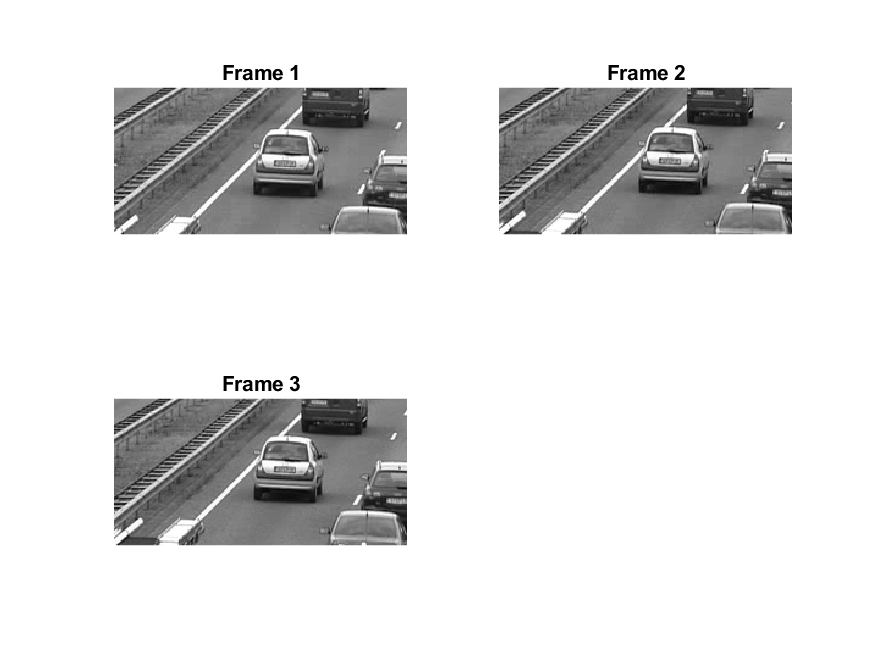
\includegraphics[width=0.4\linewidth]{originalFrames.png}
    \caption{Original Frames for T = 3}
\end{figure}

\begin{figure}[htbp]
    \centering
    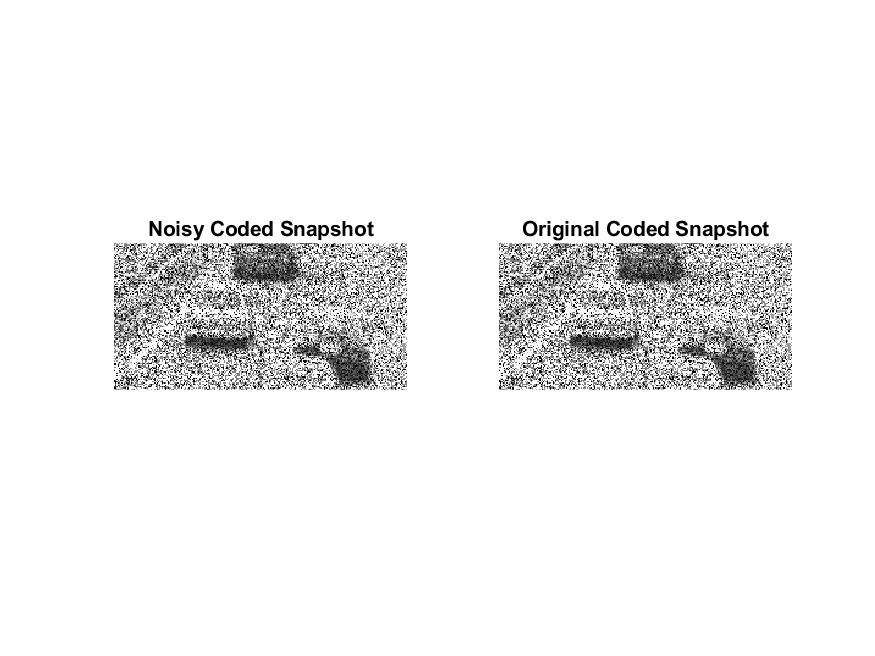
\includegraphics[width=0.4\linewidth]{noisy_coded_snapshot.png}
    \caption{Noisy coded snapshot for T = 3}
\end{figure}

\begin{figure}[htbp]
    \centering
    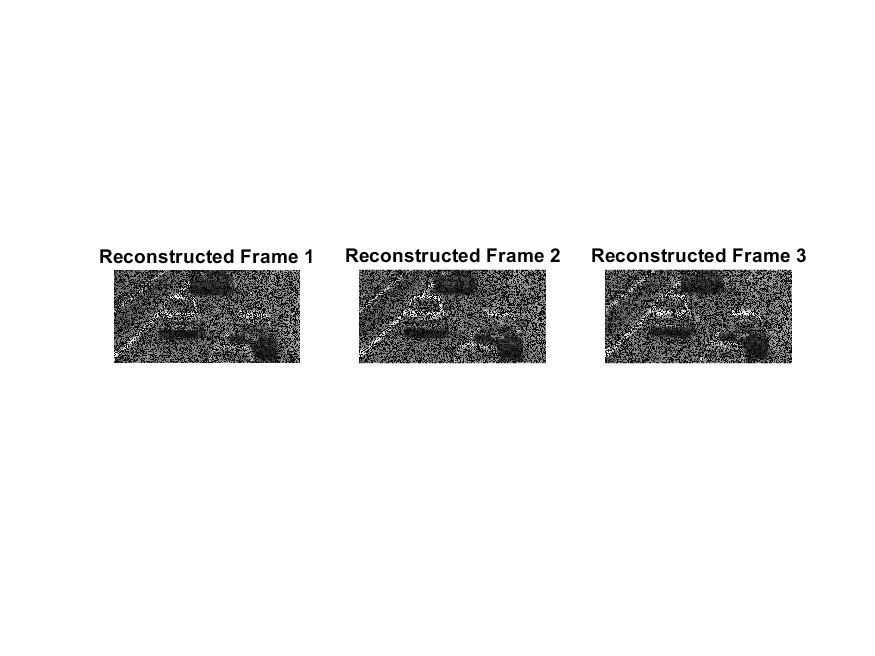
\includegraphics[width=0.4\linewidth]{reconstructed_frames.png}
    \caption{Reconstructed Frames for T = 3}
\end{figure}

\begin{figure}[htbp]
    \centering
    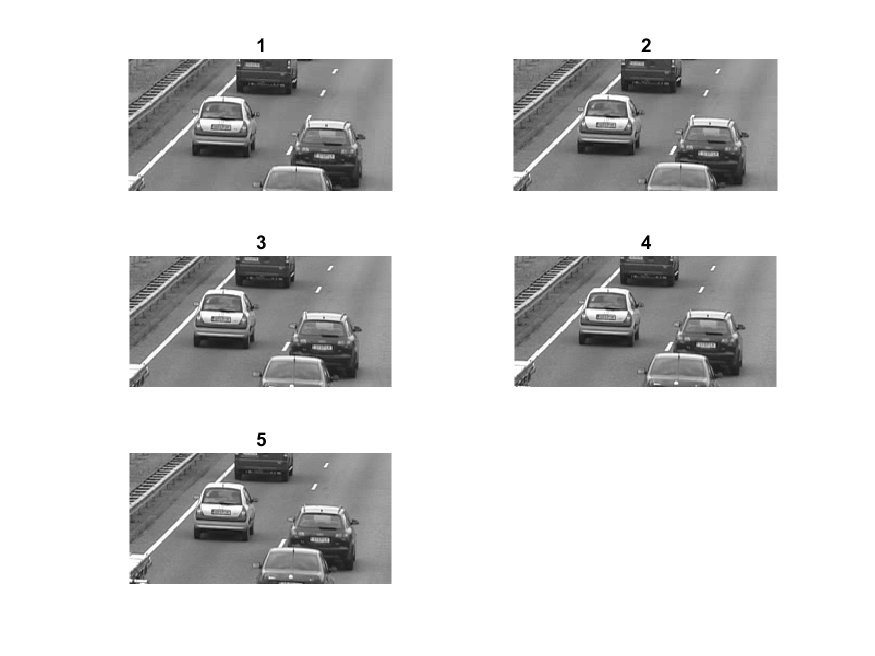
\includegraphics[width=0.4\linewidth]{original_frames_5.png}
    \caption{Original Frames for T = 5}
\end{figure}

\begin{figure}[htbp]
    \centering
    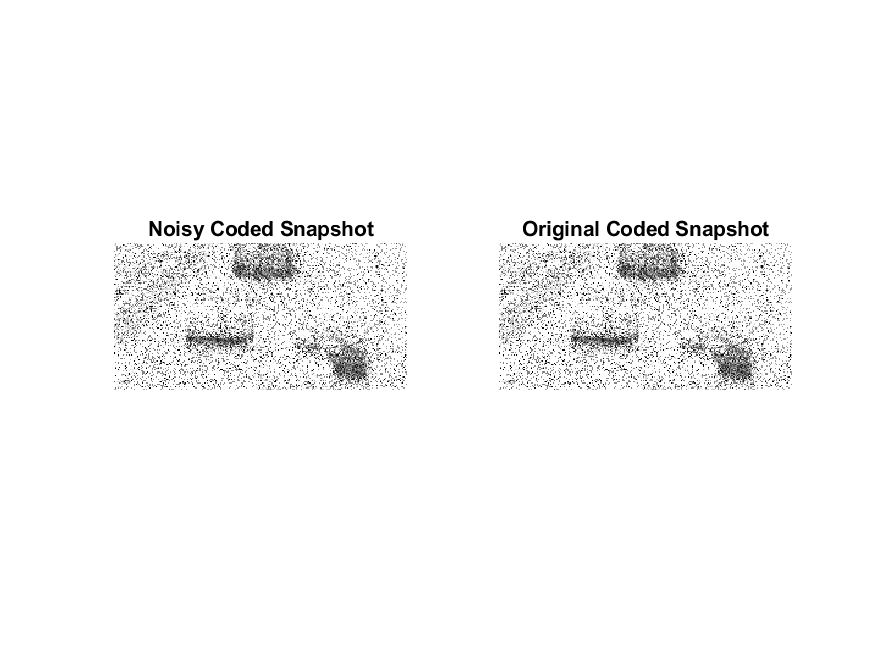
\includegraphics[width=0.4\linewidth]{noisy_coded_snapshot_5.png}
    \caption{Noisy coded snapshot for T = 5}
\end{figure}

\begin{figure}[htbp]
    \centering
    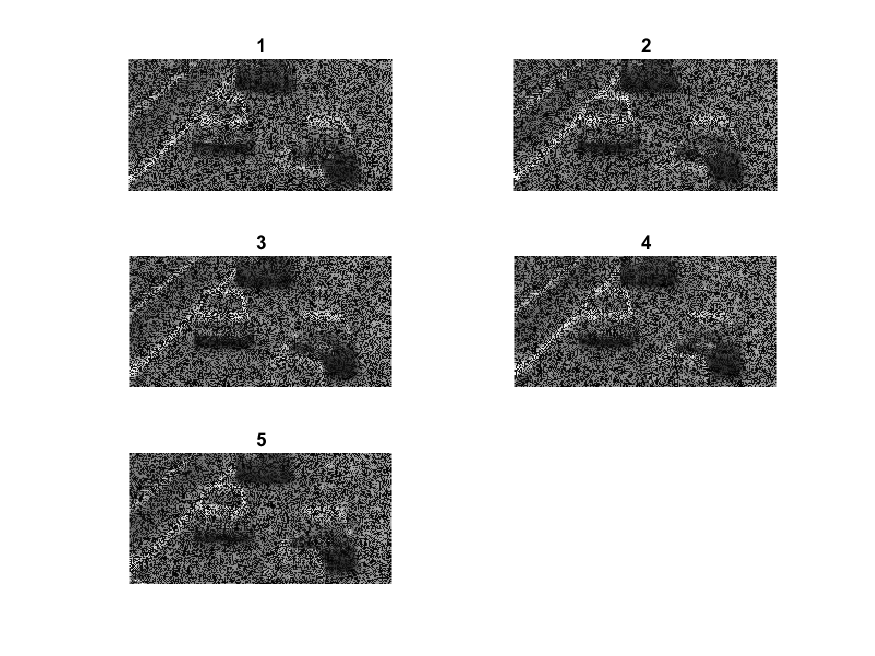
\includegraphics[width=0.4\linewidth]{reconstructed_frames_5.png}
    \caption{Reconstructed Frames for T = 5}
\end{figure}

\begin{figure}[htbp]
    \centering
    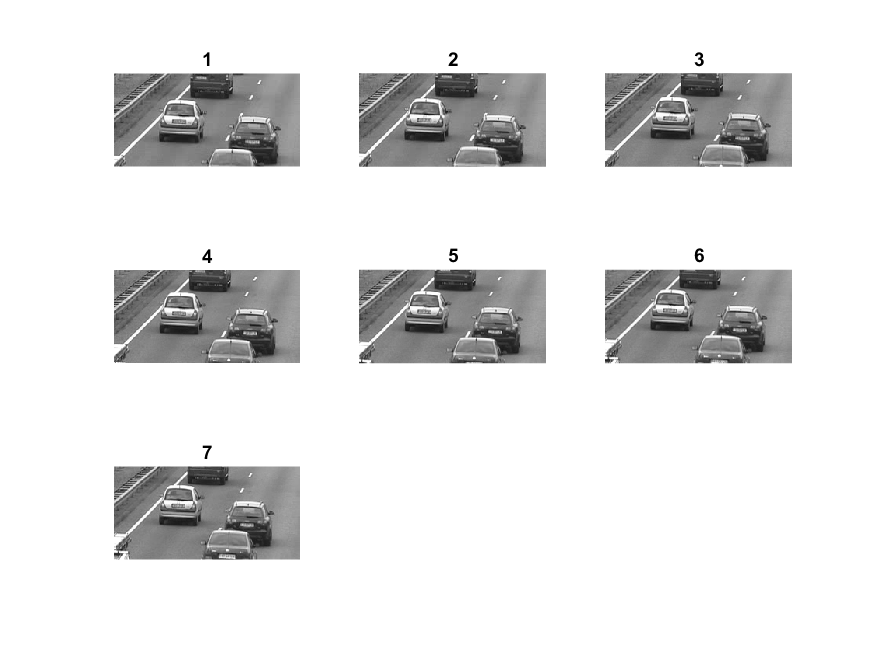
\includegraphics[width=0.4\linewidth]{original_frames_7.png}
    \caption{Original Frames for T = 7}
\end{figure}

\begin{figure}[htbp]
    \centering
    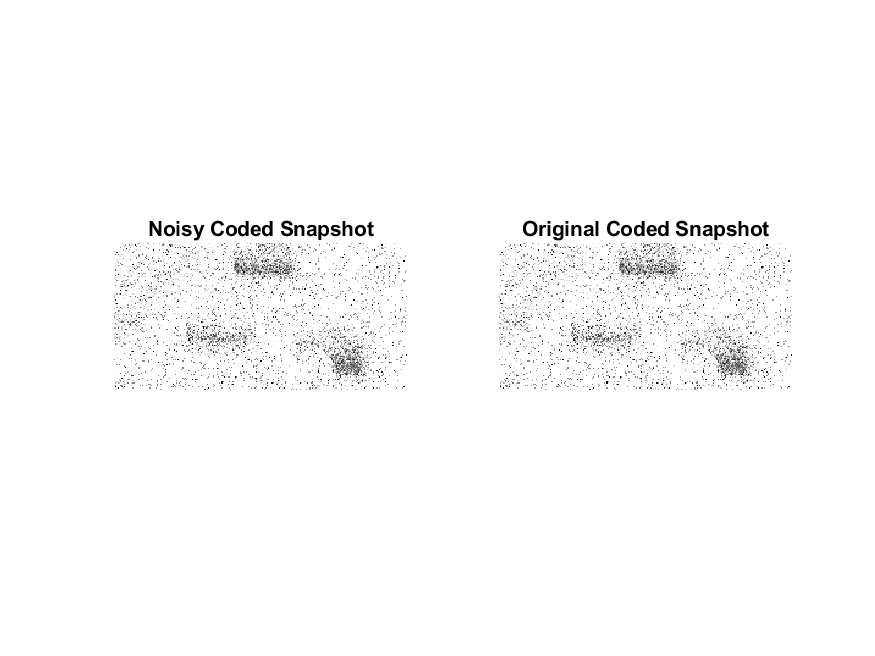
\includegraphics[width=0.4\linewidth]{noisy_coded_snapshot_7.png}
    \caption{Noisy coded snapshot for T = 7}
\end{figure}

\begin{figure}[htbp]
    \centering
    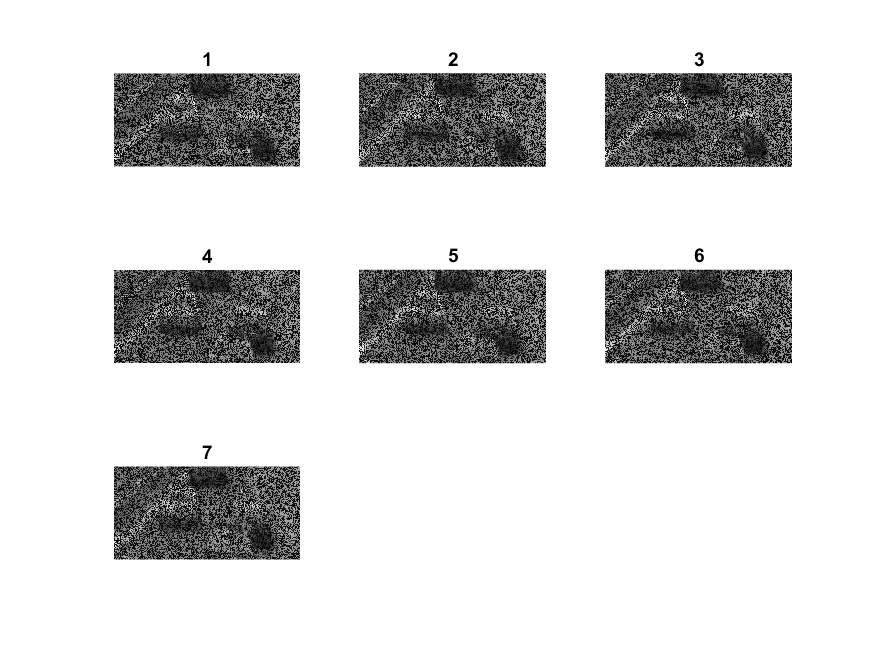
\includegraphics[width=0.4\linewidth]{reconstructed_frames_7.png}
    \caption{Reconstructed Frames for T = 7}
\end{figure}


\begin{figure}[htbp]
    \centering
    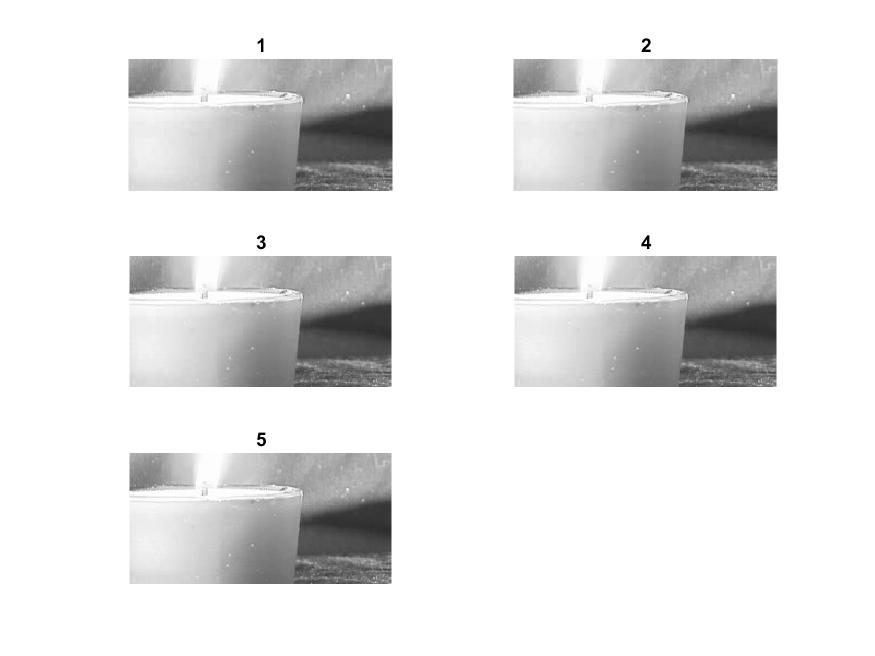
\includegraphics[width=0.4\linewidth]{original_frames_flame.png}
    \caption{Original Frames for Flame Video}
\end{figure}

\begin{figure}[htbp]
    \centering
    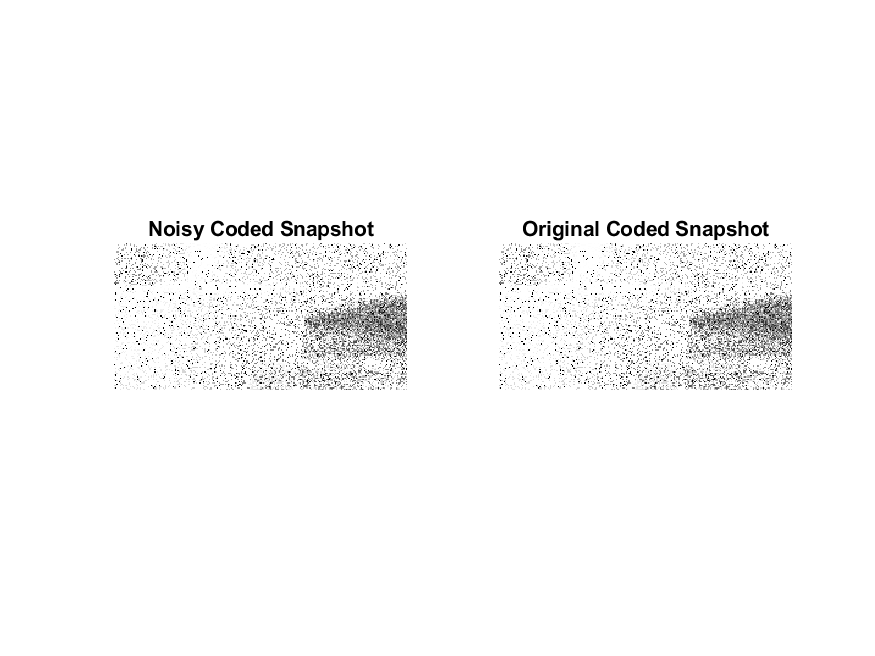
\includegraphics[width=0.4\linewidth]{noisy_coded_snapshot_flame.png}
    \caption{Noisy coded snapshot for Flames Video}
\end{figure}

\begin{figure}[htbp]
    \centering
    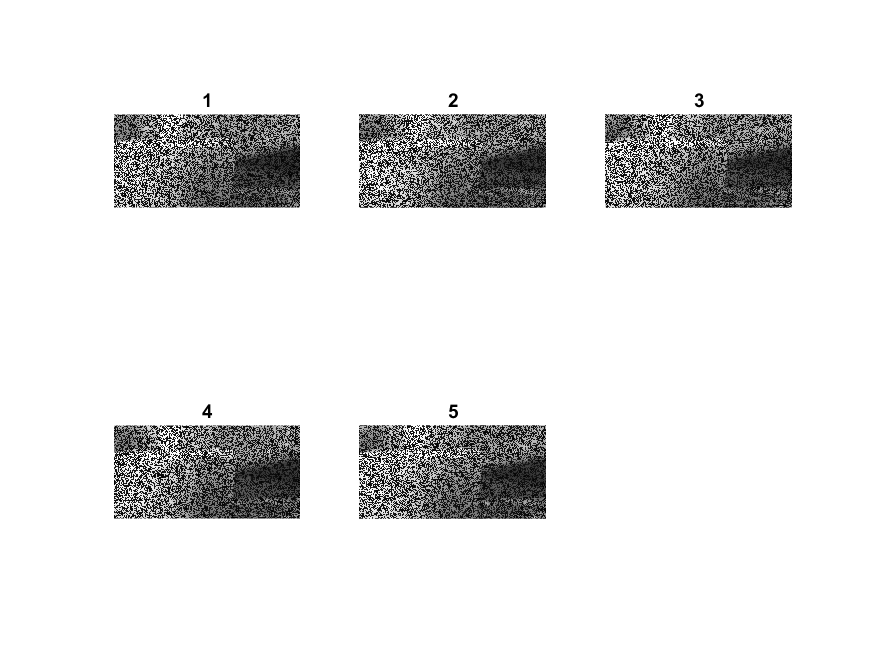
\includegraphics[width=0.4\linewidth]{reconstructed_frames_flames.png}
    \caption{Reconstructed Frames for Flames Video}
\end{figure}

\end{document}